\documentclass[12pt,twoside,letterpaper]{article}
%NOTE: This report format is 

\newcommand{\reporttitle}{Développement d'un système biométrique pour l'authentification basé sur l'iris des yeux}
\newcommand{\reportauthorOne}{François Beaulieu}
% \newcommand{\cidOne}{your id number}
\newcommand{\reportauthorTwo}{Yacine Yaddaden, Ph. D.}
% \newcommand{\cidTwo}{your id number}
\newcommand{\reporttype}{Coursework}
\bibliographystyle{plain}

% include files that load packages and define macros
%%%%%%%%%%%%%%%%%%%%%%%%%%%%%%%%%%%%%%%%%
% University Assignment Title Page 
% LaTeX Template
% Version 1.0 (27/12/12)
%
% This template has been downloaded from:
% http://www.LaTeXTemplates.com
%
% Original author:
% WikiBooks (http://en.wikibooks.org/wiki/LaTeX/Title_Creation)
%
% License:
% CC BY-NC-SA 3.0 (http://creativecommons.org/licenses/by-nc-sa/3.0/)
% 
% Instructions for using this template:
% This title page is capable of being compiled as is. This is not useful for 
% including it in another document. To do this, you have two options: 
%
% 1) Copy/paste everything between \begin{document} and \end{document} 
% starting at \begin{titlepage} and paste this into another LaTeX file where you 
% want your title page.
% OR
% 2) Remove everything outside the \begin{titlepage} and \end{titlepage} and 
% move this file to the same directory as the LaTeX file you wish to add it to. 
% Then add \input{./title_page_1.tex} to your LaTeX file where you want your
% title page.
%
%----------------------------------------------------------------------------------------
%	PACKAGES AND OTHER DOCUMENT CONFIGURATIONS
%----------------------------------------------------------------------------------------
\usepackage{ifxetex}
\usepackage{textpos}
\usepackage{natbib}
\usepackage{kpfonts}
\usepackage[letterpaper,hmargin=2.8cm,vmargin=2.0cm,includeheadfoot]{geometry}
\usepackage{ifxetex}
\usepackage{stackengine}
\usepackage{tabularx,longtable,multirow,subfigure,caption}%hangcaption
\usepackage{fncylab} %formatting of labels
\usepackage{fancyhdr}
\usepackage{color}
\usepackage[tight,ugly]{units}
\usepackage{url}
\usepackage{float}
\usepackage[francais]{babel}
\usepackage{amsmath}
\usepackage{graphicx}
\usepackage[colorinlistoftodos]{todonotes}
\usepackage{dsfont}
\usepackage{epstopdf} % automatically replace .eps with .pdf in graphics
\usepackage{natbib}
\usepackage{backref}
\usepackage{array}
\usepackage{latexsym}
\usepackage{etoolbox}

\usepackage{enumerate} % for numbering with [a)] format 



\ifxetex
\usepackage{fontspec}
\setmainfont[Scale=.8]{OpenDyslexic-Regular}
\else
\usepackage[pdftex,pagebackref,hypertexnames=false,colorlinks]{hyperref} % provide links in pdf
\hypersetup{pdftitle={},
  pdfsubject={}, 
  pdfauthor={\reportauthorOne},
  pdfkeywords={}, 
  pdfstartview=FitH,
  pdfpagemode={UseOutlines},% None, FullScreen, UseOutlines
  bookmarksnumbered=true, bookmarksopen=true, colorlinks,
    citecolor=black,%
    filecolor=black,%
    linkcolor=black,%
    urlcolor=black}
\usepackage[all]{hypcap}
\fi

\usepackage{tcolorbox}

% various theorems
\usepackage{ntheorem}
\theoremstyle{break}
\newtheorem{lemma}{Lemma}
\newtheorem{theorem}{Theorem}
\newtheorem{remark}{Remark}
\newtheorem{definition}{Definition}
\newtheorem{proof}{Proof}

% example-environment
\newenvironment{example}[1][]
{ 
\vspace{4mm}
\noindent\makebox[\linewidth]{\rule{\hsize}{1.5pt}}
\textbf{Example #1}\\
}
{ 
\noindent\newline\makebox[\linewidth]{\rule{\hsize}{1.0pt}}
}



%\renewcommand{\rmdefault}{pplx} % Palatino
% \renewcommand{\rmdefault}{put} % Utopia

\ifxetex
\else
\renewcommand*{\rmdefault}{bch} % Charter
\renewcommand*{\ttdefault}{cmtt} % Computer Modern Typewriter
%\renewcommand*{\rmdefault}{phv} % Helvetica
%\renewcommand*{\rmdefault}{iwona} % Avant Garde
\fi

\setlength{\parindent}{0em}  % indentation of paragraph

\setlength{\headheight}{14.5pt}
\pagestyle{fancy}
\fancyfoot[ER,OL]{\thepage}%Page no. in the left on
                                %odd pages and on right on even pages
\fancyfoot[OC,EC]{\sffamily }
\renewcommand{\headrulewidth}{0.1pt}
\renewcommand{\footrulewidth}{0.1pt}
\captionsetup{margin=10pt,font=small,labelfont=bf}


%--- chapter heading

\def\@makechapterhead#1{%
  \vspace*{10\p@}%
  {\parindent \z@ \raggedright %\sffamily
        %{\Large \MakeUppercase{\@chapapp} \space \thechapter}
        %\\
        %\hrulefill
        %\par\nobreak
        %\vskip 10\p@
    \interlinepenalty\@M
    \Huge \bfseries 
    \thechapter \space\space #1\par\nobreak
    \vskip 30\p@
  }}

%---chapter heading for \chapter*  
\def\@makeschapterhead#1{%
  \vspace*{10\p@}%
  {\parindent \z@ \raggedright
    \sffamily
    \interlinepenalty\@M
    \Huge \bfseries  
    #1\par\nobreak
    \vskip 30\p@
  }}
  



% %%%%%%%%%%%%% boxit
\def\Beginboxit
   {\par
    \vbox\bgroup
	   \hrule
	   \hbox\bgroup
		  \vrule \kern1.2pt %
		  \vbox\bgroup\kern1.2pt
   }

\def\Endboxit{%
			      \kern1.2pt
		       \egroup
		  \kern1.2pt\vrule
		\egroup
	   \hrule
	 \egroup
   }	

\newenvironment{boxit}{\Beginboxit}{\Endboxit}
\newenvironment{boxit*}{\Beginboxit\hbox to\hsize{}}{\Endboxit}



\allowdisplaybreaks

\makeatletter
\newcounter{elimination@steps}
\newcolumntype{R}[1]{>{\raggedleft\arraybackslash$}p{#1}<{$}}
\def\elimination@num@rights{}
\def\elimination@num@variables{}
\def\elimination@col@width{}
\newenvironment{elimination}[4][0]
{
    \setcounter{elimination@steps}{0}
    \def\elimination@num@rights{#1}
    \def\elimination@num@variables{#2}
    \def\elimination@col@width{#3}
    \renewcommand{\arraystretch}{#4}
    \start@align\@ne\st@rredtrue\m@ne
}
{
    \endalign
    \ignorespacesafterend
}
\newcommand{\eliminationstep}[2]
{
    \ifnum\value{elimination@steps}>0\leadsto\quad\fi
    \left[
        \ifnum\elimination@num@rights>0
            \begin{array}
            {@{}*{\elimination@num@variables}{R{\elimination@col@width}}
            |@{}*{\elimination@num@rights}{R{\elimination@col@width}}}
        \else
            \begin{array}
            {@{}*{\elimination@num@variables}{R{\elimination@col@width}}}
        \fi
            #1
        \end{array}
    \right]
    & 
    \begin{array}{l}
        #2
    \end{array}
    &%                                    moved second & here
    \addtocounter{elimination@steps}{1}
}
\makeatother

%% Fast macro for column vectors
\makeatletter  
\def\colvec#1{\expandafter\colvec@i#1,,,,,,,,,\@nil}
\def\colvec@i#1,#2,#3,#4,#5,#6,#7,#8,#9\@nil{% 
  \ifx$#2$ \begin{bmatrix}#1\end{bmatrix} \else
    \ifx$#3$ \begin{bmatrix}#1\\#2\end{bmatrix} \else
      \ifx$#4$ \begin{bmatrix}#1\\#2\\#3\end{bmatrix}\else
        \ifx$#5$ \begin{bmatrix}#1\\#2\\#3\\#4\end{bmatrix}\else
          \ifx$#6$ \begin{bmatrix}#1\\#2\\#3\\#4\\#5\end{bmatrix}\else
            \ifx$#7$ \begin{bmatrix}#1\\#2\\#3\\#4\\#5\\#6\end{bmatrix}\else
              \ifx$#8$ \begin{bmatrix}#1\\#2\\#3\\#4\\#5\\#6\\#7\end{bmatrix}\else
                 \PackageError{Column Vector}{The vector you tried to write is too big, use bmatrix instead}{Try using the bmatrix environment}
              \fi
            \fi
          \fi
        \fi
      \fi
    \fi
  \fi 
}  
\makeatother

\robustify{\colvec}

%%% Local Variables: 
%%% mode: latex
%%% TeX-master: "notes"
%%% End: 
 % various packages needed for maths etc.


%%%%%%%%%%%%%%%%%%%%%%%%%%%%

\begin{document}
% front page
% Last modification: 2016-09-29 (Marc Deisenroth)
% Modification for UW: 2017-05-22 (jphickey)
\begin{titlepage}

\newcommand{\HRule}{\rule{\linewidth}{0.5mm}} % Defines a new command for the horizontal lines, change thickness here


%----------------------------------------------------------------------------------------
%	LOGO SECTION
%----------------------------------------------------------------------------------------



\begin{center} % Center remainder of the page

%----------------------------------------------------------------------------------------
%	HEADING SECTIONS
%----------------------------------------------------------------------------------------


\includegraphics[width = 10cm]{uqar}\\[1.5cm] 
\textbf{\textsc{\Large INF34515-TU - Projet en informatique I}}\\[1.0cm] 
\textsc{\Large Université du Québec à Rimouski}\\[0.5cm] 
\textsc{\large Département de mathématiques, d'informatique et de génie}\\[0.95cm] 

%----------------------------------------------------------------------------------------
%	TITLE SECTION
%----------------------------------------------------------------------------------------

\HRule \\[0.4cm]
{ \huge \bfseries \reporttitle}\\ % Title of your document
\HRule \\[1.5cm]
\end{center}
%----------------------------------------------------------------------------------------
%	AUTHOR SECTION
%----------------------------------------------------------------------------------------

%\begin{minipage}{0.4\hsize}
\begin{flushleft} \large
\textit{Authors:}\\
\reportauthorOne %~(Matricule: \cidOne)\\ % Your name
\end{flushleft}
\vspace{4cm}
\makeatletter
Date: \@date 

\vfill % Fill the rest of the page with whitespace



\makeatother


\end{titlepage}




%%%%%%%%%%%%%%%%%%%%%%%%%%% table of content
%If a table of content is needed, simply uncomment the following lines
\tableofcontents
\newpage

%%%%%%%%%%%%%%%%%%%%%%%%%%%% Main document
\section{Introduction}
La sécurité informatique est un sujet qui est très d'actualité. Avec les nombreuses fuites de données des entreprises et les nombreux autres problèmes de sécurité, il est important de mettre en place des mesures de sécurité robustes. Une solution à ces problèmes est d'implémenter un système biométrique. Ces systèmes permettent d'authentifier une personne en utilisant des valeurs biométriques comme l'empreinte digitale, la voix, le visage ou l'iris. Les systèmes biométriques sont très sensibles et précis. Dans ce rapport, j'expliquerai comment j'ai développé un système biométrique basé sur l’iris de l’œil.
\cite{ref_06}

\section{Système biométrique basé sur l’iris de l’œil}

Un système biométrique basé sur l'iris de l'oeil comporte plusieurs différentes étapes. Ce processus débute avec une base de données d'iris, ensuite, on procède au pré-traitement, à l'extraction des caractéristiques, à la réduction de dimensionnalité et on termine avec le processus de classification. 

\begin{center}
    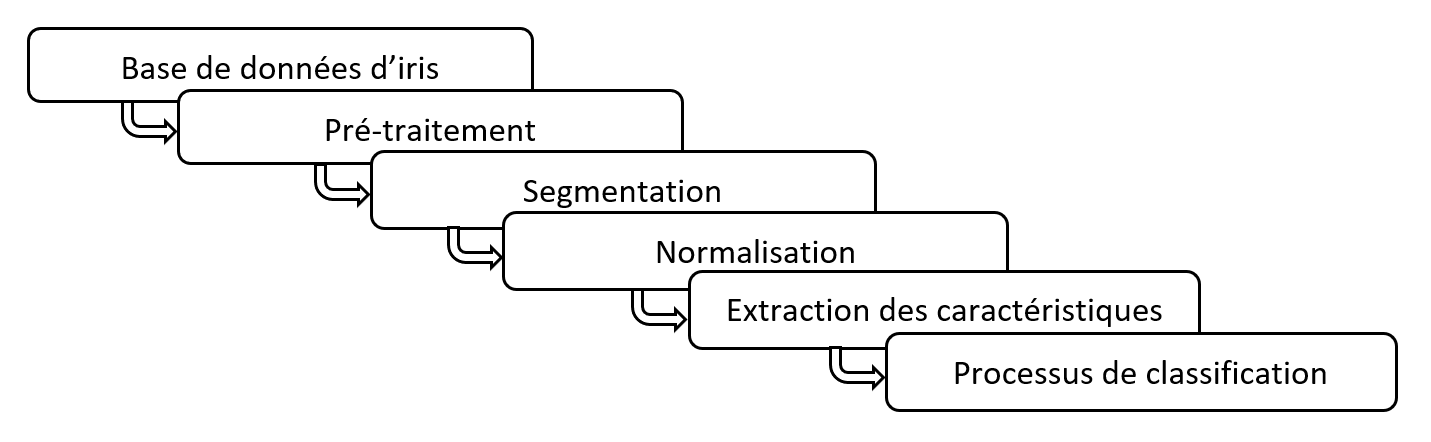
\includegraphics[width = 14cm]{schema}
\end{center}

Le processus de création d'un système biométrique basé sur l'iris de l'oeil sera détaillé dans ce qui suit.

\subsection{Base de données d’iris}
Le choix de la base de données d’iris est très important. La qualité des images peut influencer l’analyse des images. Il existe plusieurs bases de données disponibles sur internet.
\\~\\
Les éléments pouvant influencer la qualité des images sont les suivants :
\begin{itemize}
    \item Les sources de lumière
    \item Lentilles
    \item Capteur
    \item Unité de contrôle
\end{itemize}
\cite{ref_01}\cite{ref_06}
\ \\~\\
La base de données utilisée pour ce projet est « MMU iris dataset ». La base de données de « Multimedia University » (MMU1) est une base de données publique composée d'images d'oeil pour l'entraînement de modèles de système biométrique basé sur l'iris de l'oeil. Cet ensemble de données se compose de 5 images de l'iris gauche et droit de 46 personnes, pour un total de 460 images avec quelques fichiers vides.\cite{ref_05}

\subsection{Pré-traitement}
Ce processus consiste à enlever certains artefacts contenus dans les images d’origine, afin d’augmenter la précision de la reconnaissance de l’iris. Parmi les traitements pour retirer ces artefacts, on retrouve la suppression du bruit, la suppression du flou, la suppression des reflets, l’étirement du contraste, la suppression de l’occlusion des cils et la correction de l'angle du regard. Dans le pré-traitement, on doit aussi convertir les images couleurs en gris.\cite{ref_01}\cite{ref_06}


\subsubsection{Segmentation}
La segmentation de l’iris consiste à la détection de toutes les frontières de l’iris et de la pupille. C’est l’extraction de la région d’intérêt. Les techniques « Edge detection » et « Hough Transform » sont très populaires pour la segmentation de l’iris. 
\\~\\
Pour ce projet, j'ai utilisé la technique « Hough Transform » de « scikit-image ». « Hough Transform » dans sa forme la plus simple est une méthode pour détecter des lignes droites, mais elle peut également être utilisée pour détecter des cercles ou des ellipses. Pour détecter un cercle, on fournit un intervalle de rayons plausibles. Pour chaque rayon, des cercles sont extraits et on garde seulement les meilleurs candidats.\cite{ref_04}

\subsubsection{Normalisation}
La normalisation consiste à transformer l’iris circulaire en rectangle pour faciliter l’extraction des caractéristiques. « Daugman’s Rubber Sheet Model » est une méthode de normalisation utilisée pour la reconnaissance de l’iris.\cite{ref_01}\cite{ref_06}
\\~\\
Pour ce projet, j'ai utilisé la méthode « Warp Polar » de « scikit-image » pour transformer l'iris détecté à l'étape précédente en rectangle. Ensuite, j'ai retiré la partie noire (la pupille) de l'image rectangulaire. Pour ce faire, j'ai retiré toutes les lignes de l'image qui contenait 50\% ou plus de pixel avec des valeurs inférieures à (45, 45, 45).

\subsection{Extraction des caractéristiques}
L’extraction des caractéristiques consiste à représenter les caractéristiques de texture, afin de différencier les iris durant le processus de classification.\cite{ref_01}\cite{ref_06}

\subsubsection{GLCM}
Pour l’extraction des caractéristiques de l’iris, on peut utiliser la méthode GLCM (Gray-Level Co-occurrence Matrix). GLCM est une méthode statistique de second ordre pour l'analyse de texture. Les caractéristiques qui résultent des statistiques au premier ordre renseignent sur la répartition des niveaux de gris de l'image. Cependant, ils n'incluent aucune information sur les positions relatives des différents gris au sein de l'image. Les statistiques de second ordre sont utilisées pour fournir ces informations, où les pixels sont pris en compte par paires. Les statistiques du deuxième ordre et des ordres supérieurs prédisent deux valeurs de pixel ou plus l'une de l'autre à des emplacements particuliers. Les matrices de cooccurrence de niveau de gris sont des exemples de caractéristiques de second ordre de texture statique. La matrice décrit le nombre d’occurrences d’une paire (I, J) où I est le niveau de gris d’un pixel et J est le niveau de gris d’un pixel distants ou décalés de l’autre pixel (situé à 0°, 45°, 90° ou 135° du premier). Le nombre d’occurrences sera situé à la case (I, J) de la matrice GLCM.
\\~\\
De nombreuses caractéristiques de texture peuvent être identifiées à partir de la matrice GLCM. En voici quelques-unes:
\begin{itemize}
    \item \textbf{Contraste}: Évalue la variation locale du niveau de gris dans les valeurs d'intensité des pixels
    \item \textbf{Énergie}: Le nombre de paires répétées est calculé. L'énergie doit être élevée si les paires de pixels répétées sont élevées.
    \item \textbf{Entropie}: Décrit le degré de hasard nécessaire à la compression d'image.
    \item \textbf{Homogénéité}: Teste si les paires de pixels sont homogènes. L'homogénéité est supposée être élevée si les valeurs des pixels de chaque paire de pixels sont identiques.
    \item \textbf{Corrélation}: Fournit une connexion dans la paire de pixels entre les deux pixels. La corrélation est supposée être vitale si les niveaux de gris des paires de pixels sont fortement corrélés.
\end{itemize}
\cite{ref_02}
\\~\\
Pour ce projet, j'ai utilisé la méthode « GLCM » de « scikit-image » pour créer la matrice GLCM à partir de l'image de l'iris.
\\~\\
Voici un exemple de résultat de la matrice GLCM de l'iris d'un oeil:

\begin{center}
    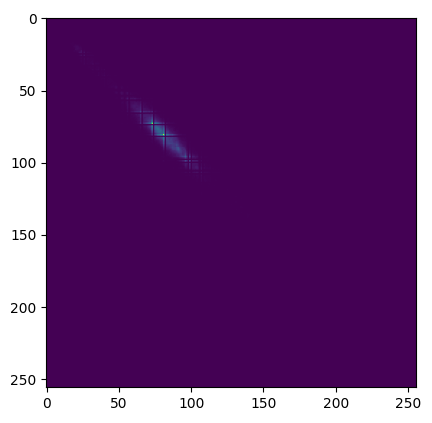
\includegraphics[width = 12cm]{glcm}
\end{center}

\subsection{Réduction de la dimensionnalité}
La réduction de la dimensionnalité est un processus qui consiste à réduire considérablement le nombre de caractéristiques pour faciliter le processus d’entraînement. La PCA est une technique qui permet de réduire la dimensionnalité.

\subsubsection{PCA}
L'analyse en composantes principales (PCA) est de loin l'algorithme de réduction de dimensionnalité le plus populaire. Cet algorithme identifie d'abord l'hyperplan le plus proche des données, puis projette les données sur celui-ci. Avant de pouvoir projeter les données sur l’hyperplan de dimension inférieure, on doit choisir le bon hyperplan. On doit donc choisir le bon axe avant de faire la projection des données. Dépendamment de l’axe choisi sur l’hyperplan, on peut conserver le plus possible la variance ou seulement la conserver faiblement. En conservant le plus la variance, on perdra le moins d’informations possible. L’objectif du PCA sera donc de conserver le plus de variance pour garder le plus d’informations possible. Le PCA identifiera l’axe qui représente la plus grande quantité de variance dans l'ensemble d'apprentissage. Ensuite, il trouvera l’axe qui représente la plus grande quantité de variance restante et ainsi de suite. Il trouvera autant d’axes que le nombre de dimensions de l’ensemble de données. Donc, pour deux dimensions, il identifiera 2 axes.
\cite{ref_03}
\\~\\
Pour ce projet, j'ai transformé chaque matrice 2D GLCM de chaque iris en un vecteur 1D grâce à la méthode « flatten » de « numpy ». Par la suite, j'ai ajouté tous les vecteurs 1D à un tableau.  Ensuite, j'ai appliqué la méthode « PCA » de « scikit-learn » sur le tableau de vecteurs.

\subsection{Processus de classification}
Le processus de classification est la dernière étape du système de reconnaissance. Il consiste à trouver le degré de similarité entre une image test et une image dans la base de données. Il permet de détecter si la personne est dans la base de données ou si c’est un imposteur.\cite{ref_01}\cite{ref_06}
\\~\\
Il existe de nombreuses techniques pour classifier les données. Une de ces techniques est la validation croisée. La validation croisée consiste à séparer les données en, par exemple, 10 sous-groupes aléatoires pour l'entraînement. Ensuite, on entraîne et évalue les données 10 fois en choisissant 9 des sous-groupes pour l'entraînement et le dernier pour l'évaluation.\cite{ref_03} Il y a aussi la méthode des k voisins les plus proches (k-NN). Elle consiste à trouver les k échantillons dont l'entrée est la plus proche d'une nouvelle entrée.

\section{Conclusion}

\newpage
\bibliography{project_report_v1.0}


\end{document}